\documentclass[10pt]{article}
\usepackage[utf8]{inputenc}
\usepackage[T1]{fontenc}
\usepackage{hyperref}
\hypersetup{colorlinks=true, linkcolor=blue, filecolor=magenta, urlcolor=cyan,}
\urlstyle{same}
\usepackage{amsmath}
\usepackage{amsfonts}
\usepackage{amssymb}
\usepackage[version=4]{mhchem}
\usepackage{stmaryrd}
\usepackage{caption}
\usepackage{graphicx}
\usepackage[export]{adjustbox}
\graphicspath{ {./images/} }
\usepackage{multirow}

\title{The Economic Costs of Conflict: A Case Study of the Basque Country }

\author{By Alberto Abadie and Javier Gardeazabal*}
\date{}


%New command to display footnote whose markers will always be hidden
\let\svthefootnote\thefootnote
\newcommand\blfootnotetext[1]{%
  \let\thefootnote\relax\footnote{#1}%
  \addtocounter{footnote}{-1}%
  \let\thefootnote\svthefootnote%
}

%Overriding the \footnotetext command to hide the marker if its value is `0`
\let\svfootnotetext\footnotetext
\renewcommand\footnotetext[2][?]{%
  \if\relax#1\relax%
    \ifnum\value{footnote}=0\blfootnotetext{#2}\else\svfootnotetext{#2}\fi%
  \else%
    \if?#1\ifnum\value{footnote}=0\blfootnotetext{#2}\else\svfootnotetext{#2}\fi%
    \else\svfootnotetext[#1]{#2}\fi%
  \fi
}

\begin{document}
\maketitle
\captionsetup{singlelinecheck=false}


\begin{abstract}
This article investigates the economic effects of conflict, using the terrorist conflict in the Basque Country as a case study. We find that, after the outbreak of terrorism in the late 1960's, per capita GDP in the Basque Country declined about 10 percentage points relative to a synthetic control region without terrorism. In addition, we use the 1998-1999 truce as a natural experiment. We find that stocks of firms with a significant part of their business in the Basque Country showed a positive relative performance when truce became credible, and a negative relative performance at the end of the cease-fire. (JEL D74, G14, P16)
\end{abstract}

Political instability is believed to have strong adverse effects on economic prosperity. However, to date, the evidence on this matter is scarce, probably because it is difficult to know how economies would have evolved in absence of political conflicts.

This article investigates the economic impact of conflict, using the terrorist conflict in the Basque Country as a case study. The Basque conflict is especially interesting from an economic perspective. At the outset of terrorist activity in the early 1970's, the Basque Country was one of the richest regions in Spain, occupying the third position in per capita GDP (out of 17 regions). In the late 1990's, after 30 years

\footnotetext{\begin{itemize}
  \item Abadie: John F. Kennedy School of Government, Harvard University, 79 John F. Kennedy Street, Cambridge, MA 02138 (e-mail: \href{mailto:alberto_abadie@harvard.edu}{alberto\_abadie@harvard.edu}); Gardeazabal: Departamento Fundamentos del Análisis Económico II, Universidad del País Vasco, Avenida Lehendakari Aguirre 83, 48015 Bilbao, Spain (e-mail: jepgamaj@ \href{http://bs.ehu.es}{bs.ehu.es}). We thank Josh Angrist, Esther Duflo, Jim Heckman, Miguel Hernán, Miguel Angel Martínez, Adolfo de Motta, Dani Rodrik, Gonzalo Rubio, Emmanuel Saez, Todd Sandler, Jim Stock, Jaume Ventura, Luis Viceira, Richard Zeckhauser, and seminar participants at CEMFI, Chicago, Harvard/MIT, the University of California-Santa Cruz, and the 2001 Summer School on Polarization and Conflict in San Sebastian for helpful comments and discussions. Thanks also go to an anonymous referee for helpful and constructive suggestions. David López-Salido, Mikel Tapia, and Fernando Tusell helped us obtain the financial data. Henry Aray, Francisco Blanch, Sara Piccicuto, and Elena Zoido provided expert research assistance and contributed comments. Gardeazabal thanks the Department of Economics at the University of California-Santa Cruz for its hospitality while part of this work was carried out.
\end{itemize}
}
of terrorist and political conflict, the Basque Country had dropped to the sixth position in per capita GDP. ${ }^{1}$ During that period, terrorist activity by the Basque terrorist organization ETA resulted in almost 800 deaths. Basque entrepreneurs and corporations had been specific targets of violence and extortion (including assassinations, robberies, and kidnappings-for-ransom). Not surprisingly, the economic downturn suffered by the Basque economy during those years has been attributed, at least partially, to the effect of terrorism. However, little research has been carried out to assess the economic effects of the conflict. ${ }^{2}$

This type of study is difficult. On the one hand, a pure time-series analysis of the severity of terrorism and the evolution of the Basque economy will be contaminated by the economic downturn which Spain suffered during the second half of the 1970's and the first half of the 1980's, at the peak of terrorist activity. On the other hand, at the outset of terrorism, the Basque Country differed from other Spanish regions in characteristics that are thought to be related to potential for economic growth. Therefore, a simple comparison of the evolution of the Basque economy and the economy of the rest of Spain would not only reflect the effect of terrorism but also the effect of pre-terrorism differences in economic growth determinants.

\footnotetext{${ }^{1}$ See Fundación BBV (1999).\\
${ }^{2}$ Notable exceptions are Walter Enders and Todd Sandler $(1991,1996)$, who study the effects of terrorism on tourism and foreign direct investment in Spain.
}Our analysis rests on two different strategies. First, we use a combination of other Spanish regions to construct a "synthetic" control region which resembles relevant economic characteristics of the Basque Country before the outset of Basque political terrorism in the late 1960's. The subsequent economic evolution of this "counterfactual" Basque Country without terrorism is compared to the actual experience of the Basque Country. We find that, after the outbreak of terrorism, per capita GDP in the Basque Country declined about 10 percentage points relative to the synthetic control region. Moreover, this gap seemed to widen in response to spikes in terrorist activity. The second part of this study uses the unilateral truce declared by ETA in September 1998 as a natural experiment to estimate the effects of the conflict. If the terrorist conflict was perceived to have a negative impact on the Basque economy, stocks of firms with a significant part of their business in the Basque Country should have shown a positive relative performance as the truce became credible, and a negative relative performance at the end of the cease-fire. We find evidence that is consistent with this conjecture using event study methods.

Most of the empirical literature on the effects of political conflict on economic variables have used cross sections of country-level data. Using a cross section of countries, Yiannis P. Venieris and Dipak K. Gupta (1986) and Alberto Alesina and Roberto Perotti (1996) concluded that political instability has a negative effect on investment and savings. Also using a cross section of countries, Robert J. Barro (1991), Paolo Mauro (1995), and Alesina et al. (1996) have argued that political instability has a negative effect on economic growth. ${ }^{3}$ A potential caveat of this literature is that part of the observed association between political conflict and economic variables across countries is thought to be created by reverse causation, since political instability is not only a cause but also an effect of fluctuations in economic variables. ${ }^{4}$ Instrumental

\footnotetext{${ }^{3}$ See also Douglas A. Hibbs (1973), Gupta (1990), John B. Londregan and Keith T. Poole (1990), Jess Benhabib and Aldo Rustichini (1996), and Daron Acemoglu and James A. Robinson (2001) on the relationship between political instability and economic variables.\\
${ }^{4}$ Conventionally, it has been argued that economic growth promotes political stability. Mancur Olson (1963) has argued,
}
variables techniques can be used to correct for reverse causation. However, the validity of instruments in cross-country regressions has often been questioned (see, e.g., N. Gregory Mankiw, 1995). Another potential shortcoming of studies based on country-level data is that political conflicts in different countries may be radically different in nature. Such heterogeneity may create problems when comparing the experiences of different countries and interpreting the results (Jonathan Temple, 1999, discusses heterogeneity issues in cross-country regressions).

Case studies, like the one presented in this article, look like the natural avenue to validate or refute the results given by cross-country studies. Heterogeneity issues are circumvented here by focusing on a particular conflict: the terrorist conflict in the Basque Country. In addition, as explained below, the Basque conflict has no direct economic motivation and, in contrast to most other violent conflicts, it does not take place in a region under particularly harsh economic conditions. Consequently, temporal variation in economic prosperity in the Basque Country during the period considered in this study is unlikely to have had a substantial effect on the intensity of terrorist activity, mitigating endogeneity issues.

\section*{I. A Brief History of ETA's Terrorist Activity}
ETA was founded in 1959 to promote the establishment of an independent Basque state. ${ }^{5}$ However, it was not until 1968 that ETA claimed its first victim. In fact, ETA did not implement large-scale terrorist activity until the\\
however, that rapid economic growth produces social dislocation and may cause political unrest. While cross-country studies have shown a positive association between poverty and political conflict (see, e.g., Paul Collier and Anke Hoeffler, 2002), Alan B. Krueger and Jitka Maleckova (2002) provide evidence that, within country, disparities in individual socioeconomic characteristics seem to be unrelated to participation in politically motivated violence.\\
${ }^{5}$ Basques are spread over the Basque Autonomous Region and Navarra in Spain, and part of the French Atlantic Pyrenees Department. The Basque Autonomous Region in Spain has been, however, the main scenario of the conflict; for the rest of the article, we use the term "the Basque Country" to refer to this region. The Basque Autonomous region is a small region with an area of 7,234 square kilometers (around 1.5 percent of the total area of Spain) and 2.1 million inhabitants in 2000 (around 5.2 percent of the total population of Spain).

\begin{table}[h]
\begin{center}
\captionsetup{labelformat=empty}
\caption{Table 1-Chronology of Eta's Terrorist Activity}
\begin{tabular}{|l|l|l|l|}
\hline
Year & Killings & Kidnappings & Event \\
\hline
1968 & 2 & 0 & First victim of ETA \\
\hline
1969 & 1 & 0 &  \\
\hline
1970 & 0 & 1 &  \\
\hline
1971 & 0 & 0 &  \\
\hline
1972 & 1 & 1 &  \\
\hline
1973 & 6 & 1 & ETA kills Franco's Prime Minister Admiral Carrero-Blanco \\
\hline
1974 & 19 & 0 &  \\
\hline
1975 & 16 & 0 & Dictator Franco dies \\
\hline
1976 & 17 & 4 &  \\
\hline
1977 & 11 & 1 & First democratic elections in Spain after Franco's death \\
\hline
1978 & 67 & 6 & Spanish Constitution approved in referendum \\
\hline
1979 & 76 & 13 & Regional Autonomy Statute for the Basque Country approved \\
\hline
1980 & 92 & 13 &  \\
\hline
1981 & 30 & 10 & Attempted military coup. Spain joins NATO \\
\hline
1982 & 37 & 8 &  \\
\hline
1983 & 32 & 5 &  \\
\hline
1984 & 32 & 0 &  \\
\hline
1985 & 37 & 3 &  \\
\hline
1986 & 41 & 3 & Spain joins European Community \\
\hline
1987 & 52 & 1 &  \\
\hline
1988 & 19 & 1 &  \\
\hline
1989 & 19 & 1 &  \\
\hline
1990 & 25 & 0 &  \\
\hline
1991 & 46 & 0 &  \\
\hline
1992 & 26 & 0 & Barcelona hosts the Summer Olympic Games \\
\hline
1993 & 14 & 1 &  \\
\hline
1994 & 13 & 0 &  \\
\hline
1995 & 15 & 1 &  \\
\hline
1996 & 5 & 2 &  \\
\hline
1997 & 13 & 1 &  \\
\hline
1998 & 6 & 0 & ETA declares indefinite cease-fire starting on September 18 \\
\hline
1999 & 0 & 0 & ETA announces the end of cease-fire on November 28 \\
\hline
2000 & 23 & 0 &  \\
\hline
\end{tabular}
\end{center}
\end{table}

Source: Spanish Ministry of Interior (2002).\\
mid-1970's. Table 1 shows the number of killings and kidnappings from 1968 to 2000. ETA's terrorist activity was low before 1973 with no more than two victims in any given year. The death toll increased sharply during the mid1970's, with an average of almost 16 victims per year in the period of 1974-1977. The blood-

\begin{table}[h]
\begin{center}
\captionsetup{labelformat=empty}
\caption{Table 2-ETA's Terrorist Activity, 1968-1997}
\begin{tabular}{lr}
\hline\hline
Deaths: &  \\
$\quad$ Basque Country & 523 \\
$\quad$ Rest of Spain & 236 \\
$\quad$ Percentage in the Basque Country & 68.91 \\
Deaths per million inhabitants per year: &  \\
$\quad$ Basque Country & 8.17 \\
$\quad$ Rest of Spain & 0.22 \\
$\quad$ Ratio Basque Country/Rest of Spain & 37.43 \\
\hline
\end{tabular}
\end{center}
\end{table}

Notes: Authors' computations from Fundación BBV (1999) and Spanish Ministry of Interior (2002). Five additional deaths in the Basque portion of the French Atlantic Pyrenees Department are not reflected in the table.\\
iest three years of ETA, 1978-1980, witnessed a total of 235 victims. In subsequent years, the number of killings decreased gradually. On average, during the 1980's, ETA's activity resulted in 39 deaths per year; this figure was reduced to 16 per year during the 1990's. The number of kidnappings during the sample period was smaller than the number of killings but evolved similarly. In September 1998, ETA declared a total and indefinite cease-fire. The ceasefire lasted approximately 14 months; in November 1999, ETA announced the end of cease-fire. In the year 2000 , ETA killed 23 people.

In order to finance its operations, ETA has used kidnappings-for-ransom, extortion, and (less frequently) robberies. The main targets of such money-raising activities have been Basque entrepreneurs, who have since begun to abandon the Basque Country in large numbers in order to escape extortion or abduction by the terrorist group. In addition, the terrorist conflict has been frequently cited as a deterrence for domestic and foreign direct investment in the Basque Country (see, e.g., The Economist, November 25, 2000).

Finally, although terrorist attacks have occurred in almost all Spanish regions, most of ETA's violent activity has been concentrated in the Basque Country. Table 2 reports deaths and deaths per million inhabitants per year caused by ETA for the period 1968-1997. Almost 70 percent of the deaths caused by ETA in Spain during 1968-1997 occurred in the Basque Country. ${ }^{6}$ This comparison becomes even more

\footnotetext{${ }^{6}$ In addition, five killings have been attributed to ETA during the same period in the Basque portion of the French Atlantic Pyrenees Department.
}\begin{table}[h]
\begin{center}
\captionsetup{labelformat=empty}
\caption{Table 3-Pre-Terrorism Characteristics, 1960's}
\begin{tabular}{|l|l|l|l|}
\hline
 & Basque Country (1) & Spain (2) & "Synthetic" Basque Country (3) \\
\hline
Real per capita GDP ${ }^{\text {a }}$ & 5,285.46 & 3,633.25 & 5,270.80 \\
\hline
Investment ratio (percentage) ${ }^{\text {b }}$ & 24.65 & 21.79 & 21.58 \\
\hline
Population density ${ }^{\text {c }}$ & 246.89 & 66.34 & 196.28 \\
\hline
\multicolumn{4}{|l|}{Sectoral shares (percentage) ${ }^{\text {d }}$} \\
\hline
Agriculture, forestry, and fishing & 6.84 & 16.34 & 6.18 \\
\hline
Energy and water & 4.11 & 4.32 & 2.76 \\
\hline
Industry & 45.08 & 26.60 & 37.64 \\
\hline
Construction and engineering & 6.15 & 7.25 & 6.96 \\
\hline
Marketable services & 33.75 & 38.53 & 41.10 \\
\hline
Nonmarketable services & 4.07 & 6.97 & 5.37 \\
\hline
\multicolumn{4}{|l|}{Human capital (percentage) ${ }^{\text {e }}$} \\
\hline
Illiterates & 3.32 & 11.66 & 7.65 \\
\hline
Primary or without studies & 85.97 & 80.15 & 82.33 \\
\hline
High school & 7.46 & 5.49 & 6.92 \\
\hline
More than high school & 3.26 & 2.70 & 3.10 \\
\hline
\end{tabular}
\end{center}
\end{table}

Sources: Authors' computations from Matilde Mas et al. (1998) and Fundación BBV (1999).\\
${ }^{\text {a }} 1986$ USD, average for 1960-1969.\\
${ }^{\mathrm{b}}$ Gross Total Investment/GDP, average for 1964-1969.\\
${ }^{\text {c }}$ Persons per square kilometer, 1969.\\
${ }^{\mathrm{d}}$ Percentages over total production, 1961-1969.\\
${ }^{\mathrm{e}}$ Percentages over working-age population, 1964-1969.\\
striking once the figures are expressed in per capita terms to reflect relative exposure to terrorism. During the period 1968-1997, ETA's activity in the Basque Country, measured as the number of deaths per inhabitant per year, was 37 times as large as in the rest of Spain. ${ }^{7}$

\section*{II. Using Other Spanish Regions to Construct a "Synthetic" Basque Country Without Terrorism}
\section*{A. Analytical Methods and Main Results}
The goal of this section is to assess the impact that terrorism has had on economic growth for the Basque Country. Table 3, in columns (1) and (2), reports values of some variables typically associated with growth potential ${ }^{8}$ for the Basque Country and Spain for the immediate pre-terrorism years. During the 1960's, relative to the whole country, the Basque Country had higher per capita income, higher investment ratio (investment/production), was more densely populated, had a higher percentage of industrial production, and a

\footnotetext{${ }^{7}$ See also Mark Kurlansky (1999) and CNN (2001) for additional background information on the Basque conflict.\\
${ }^{8}$ See, e.g., Barro and Xavier Sala-i-Martin (1995).
}
better educated labor force. As a result, a simple comparison of the economic performance of the Basque Country and the rest of Spain during the terrorism years may not only reflect the impact of terrorism, but also other pre-terrorism differences which affected subsequent economic growth.

We approach this problem by comparing the economic evolution of the Basque Country during the terrorist era with that of a weighted combination of other Spanish regions chosen to resemble the characteristics of the Basque Country before terrorism. We conceptualize such a weighted average of other Spanish regions as a "synthetic" Basque Country without terrorism, against which we can compare the actual Basque Country with terrorism. Let $J$ be the number of available control regions (the 16 Spanish regions other than the Basque Country), and $\mathbf{W}=\left(w_{1}, \ldots, w_{J}\right)^{\prime}$ a ( $J \times 1$ ) vector of nonnegative weights which sum to one. The scalar $w_{j}(j=1, \ldots, J)$ represents the weight of region $j$ in the synthetic Basque Country. Each different value for $\mathbf{W}$ produces a different synthetic Basque Country, and therefore the choice of a valid subset of control regions is embedded in the choice of the weights $\mathbf{W}$.

As said above, the weights are chosen so that the synthetic Basque country most closely re-\\
sembles the actual one before terrorism. Let $\mathbf{X}_{\mathbf{1}}$ be a ( $K \times 1$ ) vector of pre-terrorism values of $K$ economic growth predictors for the Basque Country [i.e., those values in Table 3, column (1)]. Let $\mathbf{X}_{\mathbf{0}}$ be a ( $K \times J$ ) matrix which contains the values of the same variables for the $J$ possible control regions. Let $\mathbf{V}$ be a diagonal matrix with nonnegative components. The values of the diagonal elements of $\mathbf{V}$ reflect the relative importance of the different growth predictors. The vector of weights $\mathbf{W}^{*}$ is chosen to minimize $\left(\mathbf{X}_{\mathbf{1}}-\mathbf{X}_{\mathbf{0}} \mathbf{W}\right)^{\prime} \mathbf{V}\left(\mathbf{X}_{\mathbf{1}}-\mathbf{X}_{\mathbf{0}} \mathbf{W}\right)$ subject to $w_{j} \geq 0(j=1,2, \ldots, J)$ and $w_{1}+\cdots+w_{J}=1$. The vector $\mathbf{W}^{*}$ defines the combination of nonterrorism control regions which best resembled the Basque Country in economic growth determinants at the outset of terrorism. ${ }^{9}$

Since $\mathbf{W}^{*}$ depends on $\mathbf{V}$ there is something to be said about the choice of $\mathbf{V}$. Arguably, the choice of $\mathbf{V}$ could be subjective, reflecting our previous knowledge about the relative importance of each particular growth predictor. Here, we adopt a more eclectic method, choosing $\mathbf{V}$ such that the real per capita GDP path for the Basque Country during the 1960's is best reproduced by the resulting synthetic Basque Country (see Appendix B for details).

The optimal weights, $\mathbf{W}^{*}$, are positive for two regions, Catalonia and Madrid, with values 0.8508 and 0.1492 respectively, and take value zero for the other potential controls. The selection of Catalonia and Madrid by our procedure as controls for the Basque Country is not unexpected, since a visual inspection of the data reveals that the values of the pre-terrorism characteristics for these two regions are comparable to the values of the pre-terrorism characteristics for the Basque Country. ${ }^{10}$ Column (3) of Table

\footnotetext{${ }^{9}$ This approach is closely related to statistical matching methods for observational studies (see, e.g., Paul R. Rosenbaum, 1995). The reason to restrict the weights in $\mathbf{W}$ to be nonnegative and sum to one is to prevent extrapolation outside the support of the growth predictors for the control regions. Without this restriction (and if all the diagonal elements of $\mathbf{V}$ are positive), $\mathbf{X}_{\mathbf{1}}$ would be perfectly fitted as long as the rank of $\mathbf{X}_{\mathbf{0}}$ is equal to $K$, irrespectively of how distant is $\mathbf{X}_{\mathbf{1}}$ from the elements of $\mathbf{X}_{\mathbf{0}}$. When the weights in $\mathbf{W}$ are restricted to be nonnegative and sum to one, $\mathbf{X}_{\mathbf{1}}$ cannot be perfectly fitted in general even if the rank of $\mathbf{X}_{\mathbf{0}}$ is equal to $K$. In this case, $\mathbf{X}_{\mathbf{1}}$ will be perfectly fitted only if it lies in the "support" (convex hull) of the growth predictors for the control regions.\\
${ }^{10}$ Like the Basque Country, relative to the rest of Spain during the 1960's, Catalonia and Madrid had higher levels of per capita income, population density, and human capital.
}3 reports growth predictors for the synthetic Basque Country before terrorism: $\mathbf{X}_{\mathbf{1}}^{*}=\mathbf{X}_{\mathbf{0}} \mathbf{W}^{*}$. These figures give an indication of how well the weighted combination of control regions reproduces the values of growth predictors for Basque Country before terrorism. As expected, the synthetic Basque Country looks comparable to the actual one, although some growth determinants cannot be perfectly fitted. In particular, during the 1960's, the Basque Country was the Spanish region with the highest industrial share as a percentage of total production. Therefore, a convex combination of other Spanish regions cannot perfectly reproduce the Basque sectoral shares before terrorism.

Let $\mathbf{Y}_{\mathbf{1}}$ be a ( $T \times 1$ ) vector whose elements are the values of real per capita GDP for the Basque Country during $T$ time periods. Let $\mathbf{Y}_{\mathbf{0}}$ be a ( $T \times J$ ) matrix which contains the values of the same variables for the control regions. Our goal is to approximate the per capita GDP path that the Basque Country would have experienced in the absence of terrorism. This counterfactual per capita GDP path is calculated as the per capita GDP of the synthetic Basque Country, $\mathbf{Y}_{\mathbf{1}}^{*}=\mathbf{Y}_{\mathbf{0}} \mathbf{W}^{*}$.

Figure 1 plots $\mathbf{Y}_{\mathbf{1}}$ and $\mathbf{Y}_{\mathbf{1}}^{*}$ for the period 1955-1997. The Basque Country and the synthetic control behave similarly until 1975. From 1975, when ETA's terrorist activity becomes a large-scale phenomenon, $\mathbf{Y}_{\mathbf{1}}$ and $\mathbf{Y}_{\mathbf{1}}^{*}$ diverge; the Basque Country per capita GDP takes values up to around 12 percent below those of the synthetic control. The gap in per capita GDP seems to decrease at the end of the period, taking values around 8 or 9 percent in 19951997. Overall, Figure 1 suggests a 10 -percent loss in per capita GDP due to terrorism for the 1980's and 1990's.

Statistical inference on the effect of terrorism on the economy can now be carried out by looking at the relationship between the per capita GDP gap (synthetic vs. actual Basque Country) and the intensity of terrorism in the Basque Country during the sample period. Since production factors are fixed in the short run, we

\footnotetext{In addition, Catalonia and the Basque Country were the two Spanish regions with highest shares of industrial production. As a robustness exercise, we checked that small perturbations to $\mathbf{V}$ do not alter the results substantively, even when they occasionally produce small positive weights for regions other than Catalonia and Madrid.
}\begin{figure}[h]
\begin{center}
  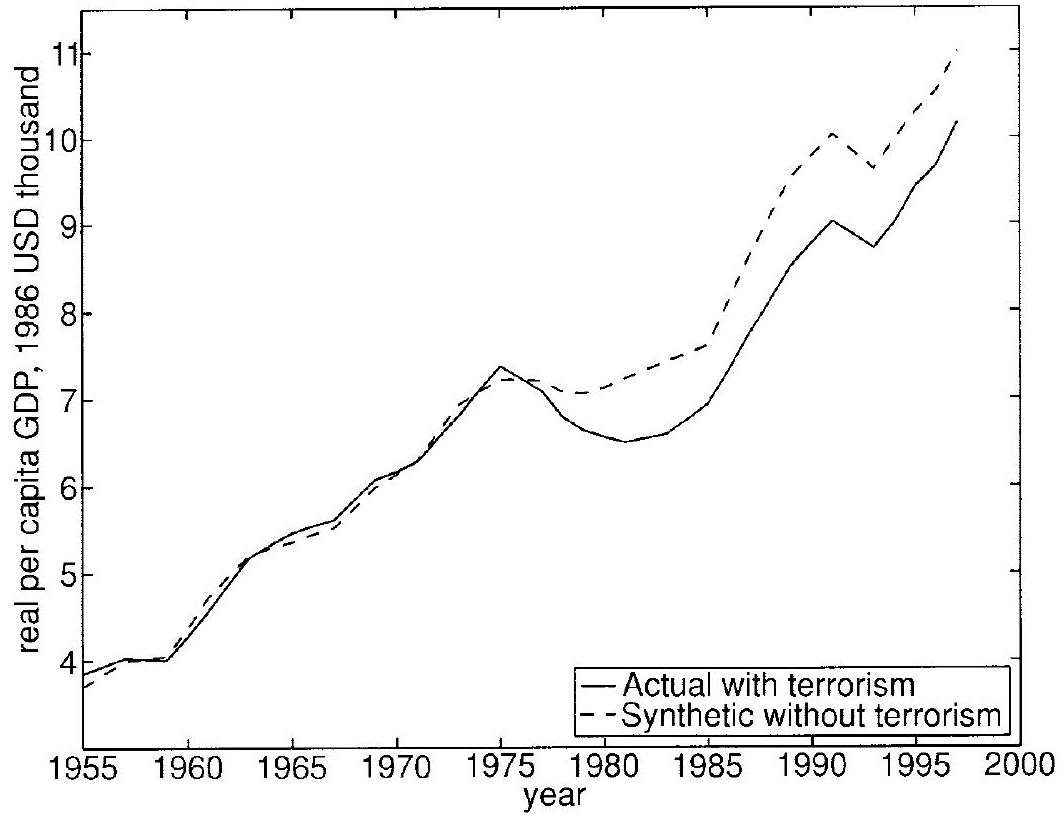
\includegraphics[alt={},max width=\textwidth]{9b44a171-0b11-4934-8139-812bee0932fe-06_820_1064_155_292}
\captionsetup{labelformat=empty}
\caption{Figure 1. Per capita GDP for the Basque Country}
\end{center}
\end{figure}

\begin{figure}[h]
\begin{center}
  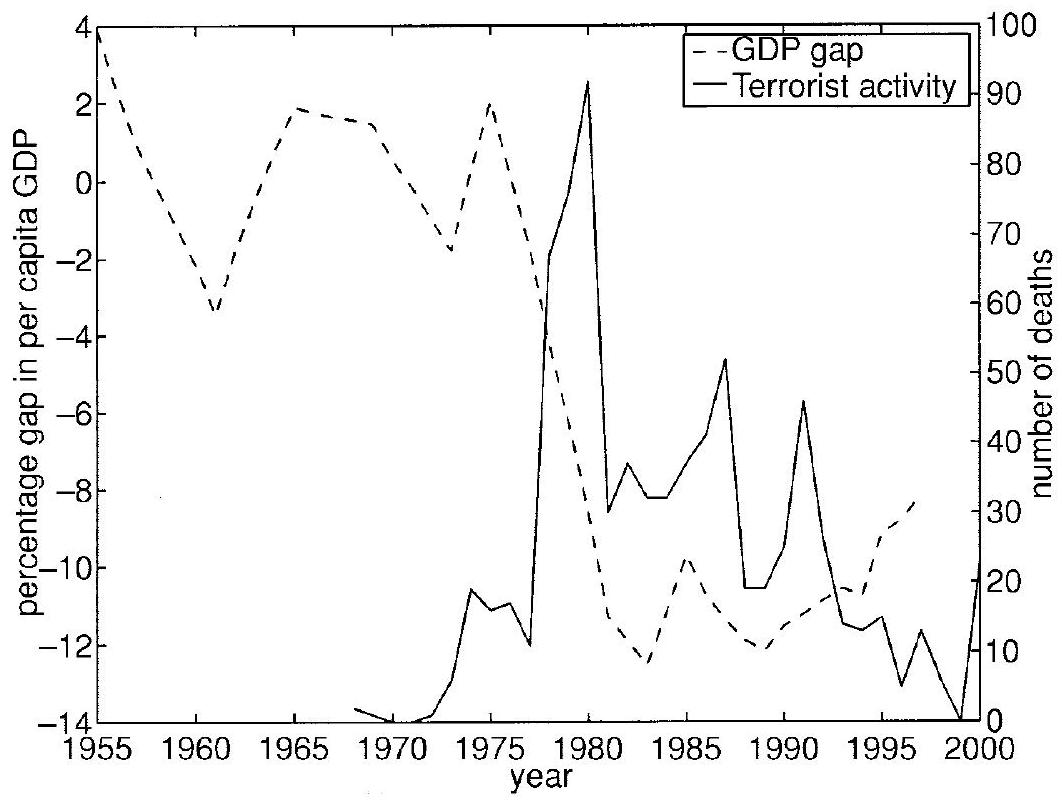
\includegraphics[alt={},max width=\textwidth]{9b44a171-0b11-4934-8139-812bee0932fe-06_802_1062_1059_294}
\captionsetup{labelformat=empty}
\caption{Figure 2. Terrorist Activity and Estimated Gap}
\end{center}
\end{figure}

expect terrorism to have a lagged negative effect on per capita GDP. In Figure 2, we plotted the per capita GDP gap, $\mathbf{Y}_{\mathbf{1}}-\mathbf{Y}_{\mathbf{1}}^{*}$, as a percentage of Basque per capita GDP, and the number\\
of deaths caused by terrorist actions (used as a proxy for overall terrorist activity). As expected, spikes in terrorist activity seem to be followed by increases in the amplitude of the

\begin{figure}[h]
\begin{center}
  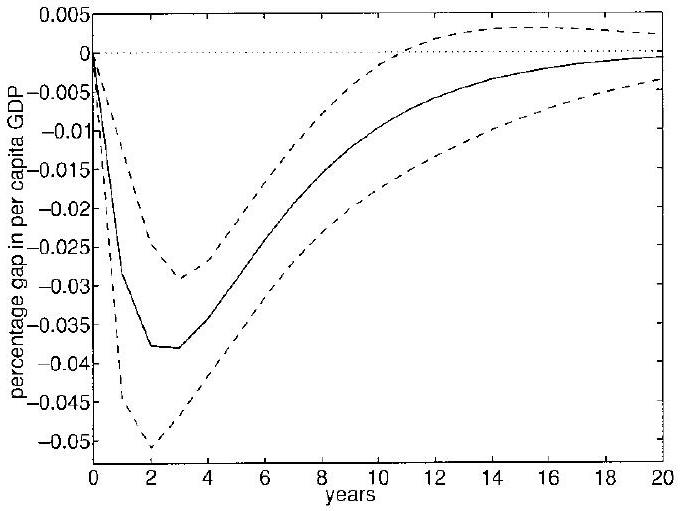
\includegraphics[alt={},max width=\textwidth]{9b44a171-0b11-4934-8139-812bee0932fe-07_511_681_152_122}
\captionsetup{labelformat=empty}
\caption{Figure 3. Impulse-Response Function for Terrorism on per capita GDP Gap and 95-Percent Confidence Intervals}
\end{center}
\end{figure}

percentage GDP gap. This pattern is confirmed by Figure 3 which shows the estimated impulseresponse function of terrorism on the GDP gap, along with 95-percent confidence intervals. The impulse-response function shows the estimated contemporaneous and lagged response of the gap to an increase of terrorist activity, proxied by an increase of one unit in the number of victims. ${ }^{11}$ The estimated effect of terrorism on the GDP gap is negative for every time lag, it is maximal after two to three years, and it decreases monotonically (in absolute value) after that. The confidence intervals for the lagged responses do not contain zero until the eleventh lag. Terrorist activity explains the GDP gap almost perfectly (see last row of Table B1 in Appendix B), and it does so in a way that is consistent with our previous beliefs about the lagged impact of terrorism on output.

\section*{B. A "Placebo Study"}
Of course, a question remains about whether the gap shown in Figure 1 truly responds to the

\footnotetext{${ }^{11}$ In other words, the impulse-response function in Figure 3 plots the dynamic multipliers of terrorism on the gap. This function was estimated using an autoregressive distributed lag model assuming no feedback effects between the gap and terrorism (see, e.g., Andrew C. Harvey, 1990). Polynomial distributed lag models were used as an alternative specification, to check the robustness of our results. Estimates based on polynomial distributed lag models produced virtually identical results. See Appendix B for details on the estimation of the impulse-response function and confidence intervals.
}
effect of terrorism or is merely an artifact of the inability of our analysis to reproduce the growth path for the Basque Country in the absence of terrorism. To address this question we performed a "placebo study," applying the method that we used to compute the gap for the Basque Country to a "nonterrorism region" (a region other than the Basque Country). The idea is to compare the economic evolution of a region similar to the Basque Country, but without high levels of terrorist activity, to the economic evolution of its synthetic version, also without high levels of terrorism. The purpose is to assess whether the gap observed for the Basque Country may have been created by factors other than terrorism.

To conduct this "placebo" study we chose Catalonia which was the region with the largest weight in the synthetic control for the Basque Country. In addition to being the region most similar to the Basque Country before terrorism in economic growth determinants (as measured using our methods), Catalonia resembles the Basque Country in many characteristics, some of which are not directly measured in our data. In particular, at the end of Franco's dictatorship, both the Basque Country and Catalonia were highly industrialized regions, and both had historical demands for self-governance, which led to the first two regional autonomy statutes of the post-Franco era in 1979. Since then, autonomy statutes have been granted to the rest of Spanish regions; however, Catalonia and the Basque Country have always been among the regions with the highest degree of political autonomy. While in both regions large fractions of the population have traditionally demanded higher levels of self-governance, Catalonia never experienced a large-scale outbreak of political terrorism.

Figure 4 shows the actual real per capita GDP path for Catalonia and the one implied by a "synthetic Catalonia" constructed as a weighted combination of other Spanish regions (excluding the Basque Country) as explained above. The weighted combination of Spanish regions reproduces per capita GDP for Catalonia with high accuracy up to the late 1980's. During 1990-1997 Catalonia outperformed the synthetic control by around 4 percent in per capita GDP. This gap does not come as a surprise if we consider the heavy investments and economic expansion that Catalonia experienced during that period as a result of the 1992 Summer Olympic Games hosted in Barcelona. Since

\begin{figure}[h]
\begin{center}
  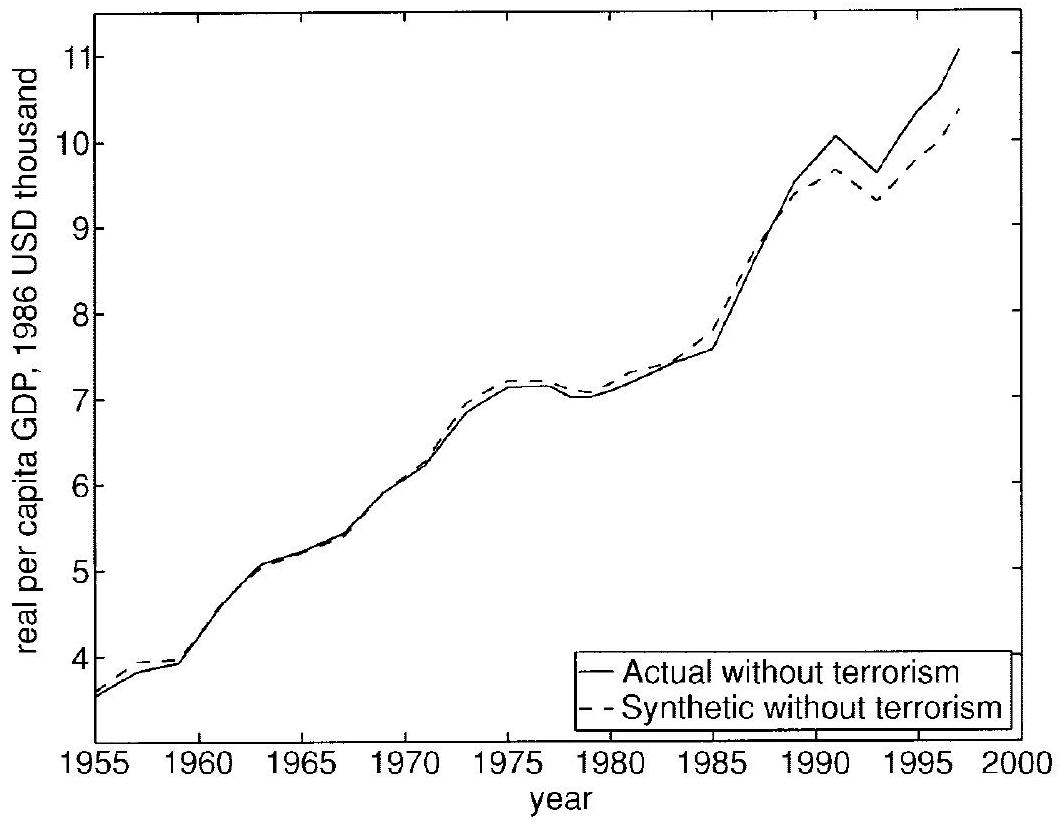
\includegraphics[alt={},max width=\textwidth]{9b44a171-0b11-4934-8139-812bee0932fe-08_823_1062_150_294}
\captionsetup{labelformat=empty}
\caption{Figure 4. A "Placebo Study," per capita GDP for Catalonia}
\end{center}
\end{figure}

Catalonia is the main contributor to the synthetic control for the Basque Country, an abnormally high level of per capita GDP for Catalonia during the 1990's may artificially widen the GDP gap for the Basque Country in Figure 1. Therefore, our placebo study suggests that, while per capita GDP for Catalonia can be reasonably well reproduced by our techniques, the catch-up in per capita GDP for the Basque Country during the 1990's (relative to the synthetic control region) may have been more pronounced than what Figure 1 indicates.

\section*{C. Discussion}
As noted earlier, the Basque Country has been the main scenario of the terrorist conflict. However, ETA has also operated in other Spanish regions. Even though there is no indication that entrepreneurs have abandoned Spain as a result of the terrorist threat, Basque terrorism might have imposed a negative reputational externality on other Spanish regions, and foreign investment might have chosen alternative destinations with no terrorist conflicts. If it is in fact the case that the Basque terrorist conflict has had a negative economic effect on other Spanish regions, this effect is arguably weaker than the\\
economic effect of terrorism on the Basque Country. To the extent that the regions which form the synthetic control might have been economically hurt by the conflict, our estimated GDP gap would provide a lower bound on the economic effect of terrorism on the Basque Country economy. On the other hand, the conflict may have diverted investment from the Basque Country to other Spanish regions, artificially increasing the magnitude of the gap. However, since the size of the synthetic Basque Country is much larger than the actual Basque Country, this type of bias is arguably small. ${ }^{12}$ In the next section we show evidence that support the view that the effect of the conflict was small outside the Basque Country.

A more important criticism of the analysis in this section is that, as long as the synthetic control cannot reproduce exactly the characteristics of the Basque Country before terrorism, the GDP gap may have been created by differ-

\footnotetext{${ }^{12}$ For the 1964-1975 period, GDP for the synthetic region was 2.5 times larger than GDP for the Basque Country; this figure increased to more than 3 during the terrorism era. Furthermore, investment diverted to regions other than those in the synthetic Basque Country does not affect the validity of our analysis.
}
ences in growth predictors between the Basque Country and the synthetic control before terrorism [columns (1) and (3) in Table 3], or by other differences not reflected in our data. In particular, it might be argued that the GDP gap was caused by the higher industrial concentration in the Basque Country in the pre-terrorism years, since terrorism developed during a period of industrial decline, when many industrial plants closed. In fact, the industrial share of GDP declined 17 percentage points (from 45 percent to 28 percent) for the Basque Country during the 1964-1993 period. The industrial share of the GDP decreased 15 percentage points (from 38 percent to 23 percent) for the synthetic control during the same period. Notwithstanding the potential importance of this criticism, we believe that differences in industrial decline between the Basque Country and the synthetic control cannot fully explain the GDP gap between the two regions during the 1980's and 1990's. As discussed earlier, the GDP gap seems to respond to the intensity of the terrorist activity in the Basque Country. Such association is consistent with the interpretation that the gap was caused by terrorism, and would be left unexplained under the alternative explanation that the gap was generated by a more pronounced industrial decline in the Basque Country. ${ }^{13}$

Figure 5 graphs population series for the Basque Country, the synthetic control and Spain (the series are normalized to 100 in 1964). The population of the Basque Country and the synthetic control grew at similar rates during the late 1960's and the early and the mid-1970's, well above the rate for the whole country. In the late 1970's and early 1980's the patterns of the series changed dramatically; population growth decelerated for the synthetic Basque Country and Spain, and became negative for the Basque Country. The results on the per capita GDP gap

\footnotetext{${ }^{13}$ The connections between the oil crisis and the decline of industrial centers in Europe during the 1970's and the 1980's has been noted by Derek H. Aldcroft (1993) and others. To check that the association between the intensity of terrorism and the gap does not arise artificially from a differential effect of the oil crisis in the Basque Country, we repeated the impulse-response analysis including contemporaneous and lagged values of oil prices as additional exogenous variables. The coefficients on the oil prices variables were not statistically significant and their inclusion left the estimated impulse-response function for terrorist activity on the gap virtually unchanged.
}\begin{figure}[h]
\begin{center}
  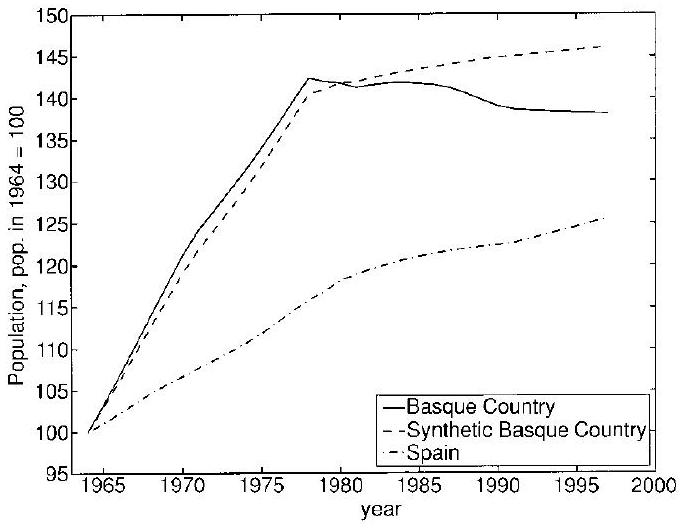
\includegraphics[alt={},max width=\textwidth]{9b44a171-0b11-4934-8139-812bee0932fe-09_529_687_148_850}
\captionsetup{labelformat=empty}
\caption{Figure 5. Population}
\end{center}
\end{figure}

presented in this section do not reflect this relative population loss in the Basque Country. Once the population dynamics are considered, the gap in per capita GDP documented in this section becomes even more striking.

Finally, it is worth noticing that the results in this section are consistent with the findings in Barro and Sala-i-Martin (1995, page 399, Figure 11.8), who document an atypically low growth rate for the Basque Country during the period 1950-1999 relative to other European regions.

\section*{III. Using ETA's 1998-1999 Truce as a Natural Experiment}
\section*{A. Analytical Methods and Main Results}
On September 16, 1998, ETA announced a cease-fire (starting on September 18, 1998). Fourteen months later, on November 28, 1999, ETA announced the end of the truce. Table 4 presents a chronology of some of the most important events related to the truce. Anecdotal evidence suggests that the truce was not perceived as credible from the beginning (note, for example, the Spanish government's reaction to the announcement of the cease-fire in Table 4, event number 4). In fact, ETA had declared other cease-fires in the past, but none of them lasted more than three months; the previous one, in 1996, had only lasted one week. ${ }^{14}$ Peace

\footnotetext{${ }^{14}$ The announcement of the cease-fire was preceded by a joint declaration subscribed by the main Basque nationalist parties calling for the end of violence and the start of
}\begin{table}[h]
\begin{center}
\captionsetup{labelformat=empty}
\caption{Table 4-Chronology of the Truce}
\begin{tabular}{|l|l|l|}
\hline
Number & Date & Event \\
\hline
1 & September 12, 1998 & Basque nationalist parties (including ETA's political wing) sign joint declaration calling for the end of violence and the start of political negotiations with the Spanish government on issues regarding sovereignty \\
\hline
2 & September 15, 1998 & Spanish Minister of Interior says the government expects "fake truce" by ETA intended to regroup and gain popular support \\
\hline
3 & September 16, 1998 & ETA calls cease-fire starting on September 18 \\
\hline
4 & September 17, 1998 & Spanish government expresses "profound skepticism" about the truce and advises caution \\
\hline
5 & October 2, 1998 & Spanish Prime Minister says ETA has yet to prove its commitment to peace, but promises changes in policy towards incarcerated ETA activists if peace consolidates \\
\hline
6 & October 24, 1998 & ETA leaders say cease-fire is "firm and serious" in BBC TV broadcast \\
\hline
7 & November 3, 1998 & Spanish government says it has authorized exploratory contacts with ETA in order to assess ETA's commitment to maintain cease-fire \\
\hline
8 & February 24, 1999 & ETA's communique pledges to maintain cease-fire and alludes to a new "hopeful climate" \\
\hline
9 & May 16, 1999 & ETA says it has maintained contacts with Spanish government \\
\hline
10 & June 2, 1999 & Spanish government confirms conversations with ETA \\
\hline
11 & August 25, 1999 & Spanish Prime Minister says that contacts with ETA have been interrupted \\
\hline
12 & August 26, 1999 & ETA confirms that the peace process is paralyzed \\
\hline
13 & August 28, 1999 & ETA's communique states that the peace process has reached a "critical stage" in which it is either concluded "or else it will rot" \\
\hline
14 & November 28, 1999 & ETA announces the end of cease-fire \\
\hline
\end{tabular}
\end{center}
\end{table}

prospects became more realistic as time passed without terrorist actions and the Spanish government confirmed contacts with ETA. Three months before the end of the truce the situation deteriorated as the Spanish government announced that the process was paralyzed.

If financial markets are efficient, asset prices should reflect all available information and, thus, react only to new information. Therefore, if the terrorist conflict was perceived to have a negative impact on the Basque economy, Basque stocks (stocks of firms with a significant part of their business in the Basque Country) should have shown a positive performance relative to non-Basque stocks (stocks of firms without a significant part of their business in the Basque Country) as the truce became credible. Similarly, Basque stocks should have performed poorly, relative to non-Basque stocks, at the end of the truce. In this section, we use the method of event study to explore these questions.\\
political negotiation (event 1 in Table 4). This declaration and the subsequent announcement of the truce were interpreted by many nonsubscribing parties as maneuvers of Basque nationalist parties to create a united front to pursue independence.

A challenge with this exercise is that there is no obvious way to classify stocks into the Basque/ non-Basque categories. A classification that relies solely on companies' registered addresses seems problematic. Registered addresses are sometimes chosen for historic, convenience, or tax-related reasons and do not necessarily imply that the company has an important presence in the area. Unfortunately, data on geographical location of firms' activities are rarely available. To solve this problem we adopted a simple and direct approach. Since what is relevant for our event study is which companies were perceived by the markets as carrying a significant part of their business in the Basque Country, we asked a group of market analysts at a certain Basque financial institution to produce this classification for us. We used this information to divide stocks into Basque stocks and non-Basque stocks. Again, the idea is to label firms which have a large part of their business in the Basque Country as Basque stocks, even if they are not located in the Basque Country. All other firms with little exposure in the Basque Country were labeled as non-Basque stocks. ${ }^{15}$

We collected series of daily stock returns

\footnotetext{${ }^{15}$ The list of Basque and non-Basque stocks used for the analysis is provided in Appendix B, Table B2.
}\begin{table}[h]
\begin{center}
\captionsetup{labelformat=empty}
\caption{Table 5-Descriptive Statistics}
\begin{tabular}{|l|l|l|l|l|l|}
\hline
\multicolumn{3}{|c|}{} & Basque & NonBasque & All \\
\hline
Number of observations &  &  & 14 & 59 & 73 \\
\hline
\multicolumn{2}{|l|}{Registered in the Basque Country} & Fraction & 0.57 & 0.00 & 0.11 \\
\hline
\multirow[t]{12}{*}{Size} & \multirow[t]{4}{*}{1998} & Mean & 412.28 & 1,999.37 & 1,695.00 \\
\hline
 &  & S.D. & 362.84 & 4,501.26 & 4,091.61 \\
\hline
 &  & Min & 117.66 & 17.01 & 17.01 \\
\hline
 &  & Max & 1,531.68 & 26,778.68 & 26,778.68 \\
\hline
 & \multirow[t]{3}{*}{1999} & Mean & 478.70 & 2,948.63 & 2,474.94 \\
\hline
 &  & S.D. & 348.46 & 7,105.34 & 6,453.67 \\
\hline
 &  & Min & 104.56 & 15.88 & 15.88 \\
\hline
 &  & Max & 1,244.64 & 45,347.23 & 45,347.23 \\
\hline
 & \multirow[t]{4}{*}{2000} & Mean & 371.43 & 3,346.84 & 2,776.21 \\
\hline
 &  & S.D. & 406.43 & 11,305.43 & 10,216.72 \\
\hline
 &  & Min & 56.20 & 9.12 & 9.12 \\
\hline
 &  & Max & 1,656.38 & 81,292.33 & 81,292.33 \\
\hline
\multirow[t]{12}{*}{Book-to-market} & \multirow[t]{3}{*}{1998} & Mean & 0.68 & 0.55 & 0.58 \\
\hline
 &  & S.D. & 0.43 & 0.34 & 0.36 \\
\hline
 &  & Min & 0.20 & 0.09 & 0.09 \\
\hline
 &  & Max & 1.65 & 1.80 & 1.80 \\
\hline
 & \multirow[t]{3}{*}{1999} & Mean & 0.72 & 0.50 & 0.54 \\
\hline
 &  & S.D. & 0.55 & 0.29 & 0.36 \\
\hline
 &  & Min & 0.14 & 0.07 & 0.07 \\
\hline
 &  & Max & 2.28 & 1.38 & 2.28 \\
\hline
 & \multirow[t]{4}{*}{2000} & Mean & 0.86 & 0.68 & 0.71 \\
\hline
 &  & S.D. & 0.46 & 0.43 & 0.44 \\
\hline
 &  & Min & 0.30 & 0.08 & 0.08 \\
\hline
 &  & Max & 1.70 & 2.26 & 2.26 \\
\hline
\end{tabular}
\end{center}
\end{table}

Source: Authors' computations from Madrid Stock Exchange online data (\href{http://www.bolsamadrid.es}{http://www.bolsamadrid.es}). Size values in millions of United States dollars. Size and book-to-market figures are for the beginning of the indicated year (last trading day of the previous year). S.D. means standard deviation.\\
for 1998, 1999, and 2000 and constructed two buy-and-hold portfolios: one composed of 14 Basque stocks and the other composed of 59 non-Basque stocks (see Appendix B for details on selection of stocks for our sample and construction of portfolios). Buy-and-hold portfolios represent the portfolio of a passive investor who constructed a value-weighted Basque or non-Basque portfolio at the beginning of our sample period. ${ }^{16}$

Table 5 contains descriptive statistics for our sample. Fifty-seven percent of the firms that compose our Basque portfolio have registered addresses in the Basque Country, while none of the non-Basque firms are registered in the Basque Country. On average, Basque firms are

\footnotetext{${ }^{16}$ The strategy of constructing portfolios of firms exposed and not exposed to certain risks is often used in event studies. See, for instance, Bong Chan Kho et al. (2000).
}
smaller and have a higher book-to-market ratio. ${ }^{17}$

In contrast with more conventional event study settings, where most of the information is revealed during short event windows, the informational content of the truce evolved gradually during a 14 -month period. Therefore, to study the effect of the truce it is important to control for long-run risk factors in stock returns. Fama and French (1993) have identified three common risk factors in stock returns, which compose the often-called Fama-French ThreeFactor Model:

\footnotetext{${ }^{17}$ Size is the market value of all outstanding shares of a common stock. The book-to-market ratio is the ratio of the book value of a stock to its market value. Size and the book-to-market ratio have been shown to explain crosssectional variation in average stock returns (see, e.g., Eugene F. Fama and Kenneth R. French, 1992).
}\begin{table}[h]
\begin{center}
\captionsetup{labelformat=empty}
\caption{Table 6-Portfolio Regressions, Fama-French Three-Factor Model}
\begin{tabular}{|l|l|l|l|l|l|}
\hline
 & Basque (1) & Non-Basque (2) & Basque (3) & Non-Basque (4) & Difference (3)-(4) \\
\hline
Constant & -0.0004 (0.0003) & 0.0001 (0.0002) & -0.0004 (0.0003) & 0.0001 (0.0002) & -0.0005 (0.0003) \\
\hline
$R^{m}$ & 0.6824 (0.0361) & 0.8103 (0.0184) & 0.6739 (0.0366) & 0.8096 (0.0186) & -0.1357 (0.0346) \\
\hline
$S M B$ & 0.3755 (0.0461) & -0.2253 (0.0234) & 0.3657 (0.0464) & -0.2260 (0.0235) & 0.5917 (0.0445) \\
\hline
HML & 0.2510 (0.0399) & -0.1418 (0.0207) & 0.2553 (0.0400) & -0.1411 (0.0207) & 0.3964 (0.0382) \\
\hline
Good News &  &  & 0.0049 (0.0021) & 0.0005 (0.0009) & 0.0044 (0.0022) \\
\hline
Bad News &  &  & -0.0017 (0.0008) & 0.0001 (0.0004) & -0.0018 (0.0009) \\
\hline
$R^{2}$ & 0.4891 & 0.9107 & 0.4966 & 0.9107 & 0.5499 \\
\hline
\end{tabular}
\end{center}
\end{table}

Notes: Heteroskedasticity-robust standard errors are in parentheses. The sample period consists of 747 trading sessions for 1998-2000.


\begin{align*}
R_{t}^{j}= & \alpha^{j}+\beta_{1}^{j} R_{t}^{m}+\beta_{2}^{j} S M B_{t}  \tag{1}\\
& +\beta_{3}^{j} H M L_{t}+A R_{t}^{j} .
\end{align*}


For the case studied here, $R_{t}^{j}$ is the excess return (over the risk-free rate) on a buy-and-hold portfolio of $j=$ Basque, non-Basque stocks on day $t, R_{t}^{m}$ is the excess return on the market portfolio at time $t, S M B_{t}$ ("small minus big") is the difference between the returns of portfolios composed by small and big size stocks at time $t$, and $H M L_{t}$ ("high minus low") is the difference between the returns of portfolios composed by high and low book-to-market stocks at time $t$.\\
$R_{t}^{m}$ represents the usual market factor in stock returns, while $S M B_{t}$ and $H M L_{t}$ are meant to capture risk factors related to size and book-tomarket equity, respectively. The residual, $A R_{t}^{j}$, is a zero mean abnormal portfolio return not explained by common risk factors. ${ }^{18}$

Columns (1) and (2) of Table 6 report the results of fitting equation (1) by ordinary least squares (OLS) to the Basque and non-Basque portfolios. The coefficients on $R_{t}^{m}, S M B_{t}$, and

\footnotetext{${ }^{18}$ See the influential article by Fama and French (1993) and Appendix B for more information about the definition and construction of these variables. Fama and French (1993) and John D. Lyon et al. (1999) discuss the use of the Fama-French Three-Factor Model to calculate longrun abnormal returns in event studies. In particular, Fama and French (1993) have argued that $S M B_{t}$ and $H M L_{t}$ absorb the size and book-to-market effects in average stock returns.
}
$H M L_{t}$ are all significant. The coefficients on $R_{t}^{m}$ are positive in both cases, whereas the coefficients on $S M B_{t}$ and $H M L_{t}$ have positive signs for the Basque portfolio and negative signs for the non-Basque portfolio. ${ }^{19}$ The residuals of the regressions are the estimated abnormal returns on the Basque and non-Basque portfolios. Abnormal returns are now suited for comparison, as they are adjusted for known risk factors. However, abnormal returns are too noisy to be visually instructive. In order to visually inspect the difference in performance of the two portfolios, abnormal returns are customarily aggregated through time. We calculate cumulative abnormal returns as the compounded abnormal return of a portfolio from the day after the announcement of the truce:

\begin{equation*}
C A R_{t}^{j}=\left(\prod_{s=1}^{t}\left\{1+A R_{s}^{j}\right\}\right)-1 . \tag{2}
\end{equation*}


Figure 6 graphs cumulative abnormal returns for the Basque and non-Basque portfolios from the announcement of the truce to the end of 1999 (the dashed vertical line around the end of

\footnotetext{${ }^{19}$ As in Fama and French (1993), we expect that returns of portfolios constructed from stocks with small market valuations and high book-to-market ratios (as the Basque portfolio) respond positively to $S M B_{t}$ and $H M L_{t}$, whereas returns of portfolios constructed from stocks with big market valuations and low book-to-market ratios (as the nonBasque portfolio) respond negatively to $S M B_{t}$ and $H M L_{t}$.
}\begin{figure}[h]
\begin{center}
  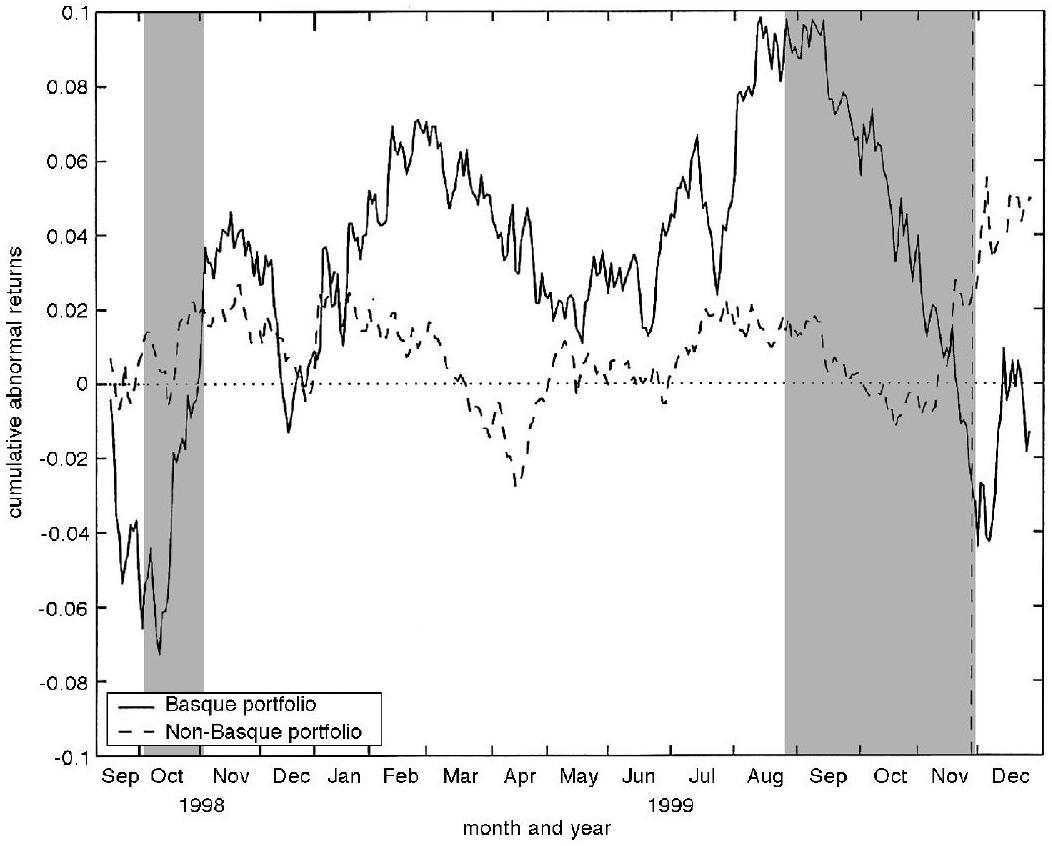
\includegraphics[alt={},max width=\textwidth]{9b44a171-0b11-4934-8139-812bee0932fe-13_846_1052_157_299}
\captionsetup{labelformat=empty}
\caption{Figure 6. Cumulative Abnormal Portfolio Returns}
\end{center}
\end{figure}

November of 1999 represents the end of the truce). The Basque portfolio outperforms the non-Basque portfolio for most of the truce period except at the beginning (when the ceasefire had not gained credibility) and at the end (when the cease-fire lost credibility).

To perform a statistical test on the effect of the truce we added two dummy variables to equation (1). Good News ${ }_{t}$ takes a value of one for the period between the trading sessions after event 5 and event 7 in Table 4, and a value of zero otherwise. Bad News ${ }_{t}$ takes a value of one for the period between the trading sessions after event 11 and event 14 in Table 4, and a value of zero otherwise. The Good News period comprises 22 trading sessions and the Bad News period 66. During the Good News period, the credibility of the truce gained ground, starting with the offer of a revision in the policy towards ETA activists in jail, if peace consolidated, by the Spanish Prime Minister (event number 5), and culminating with the announcement of the authorization of direct contacts with ETA by the Spanish government (event number 7). In contrast, the Bad News period was characterized by the collapse of the peace process, starting with the acknowledgment that contacts had been interrupted, made by the Spanish Prime

Minister (event number 11), and ending with the announcement of the end of the truce by ETA (event number 14). Columns (3) and (4) of Table 6 report the regressions including the dummy variables Good News ${ }_{t}$ and Bad $N e w s{ }_{t}$. The estimated coefficients on the dummy variables represent average daily abnormal returns during the Good News and Bad News periods for the Basque and non-Basque portfolios. As expected, for the Basque portfolio, the coefficient of Good News ${ }_{t}$ is positive and significant while the coefficient of Bad News ${ }_{t}$ is negative and also significant. For the non-Basque portfolio, the effects are small in magnitude and not statistically different from zero, which supports the view that Basque terrorism has a minor impact on the economy outside the Basque Country. The last column of Table 6 shows the result for the difference regression. The dependent variable for the difference regression is the difference in excess return between the Basque and the nonBasque portfolios. The difference regression can be interpreted as the one that corresponds to the portfolio of a passive investor who takes a long position in Basque stocks and a short position in non-Basque stocks. This regression reflects a positive abnormal performance of

Basque stocks relative to non-Basque stocks during the Good News period and a negative relative performance during the Bad News period.

The performances of the Basque and the nonBasque portfolios during the Good News and Bad News periods can be easily visualized in Figure 6. The first shaded area, around October of 1998, represents the Good News period; the second one, around September to November of 1999, represents the Bad News period. The abnormal gains in value for the Basque portfolio during the Good News period and the losses during the Bad News period are apparent. In contrast, the non-Basque portfolio experienced relatively modest abnormal changes in value during the two periods.

\section*{B. Discussion}
Notice that if most of the new information during the Good News and Bad News periods was revealed in certain trading sessions, the analysis in this section would provide conservative inference about the effect of terrorism, because the coefficients on the Good News ${ }_{t}$ and Bad News ${ }_{t}$ dummies reflect average abnormal returns during these periods. Even so, the coefficients on the Good News ${ }_{t}$ and Bad $N e w s_{t}$ dummies are statistically significant at conventional levels.

To better understand the magnitude of the effects described in this section it is useful to compound the daily effects for the Good News and Bad News periods. Compounding the 0.0044 coefficient on the Good News ${ }_{t}$ dummy over the 22 trading sessions of the Good News period, we obtain a compounded abnormal return of 10.14 percent for the Basque portfolio relative to the non-Basque portfolio. Analogous calculations yield a -11.21 -percent compounded abnormal return for the Basque portfolio relative to the non-Basque portfolio during the 66 trading sessions of the Bad News period. These are sizable differences which would be difficult to explain unless they are attributed to the differential effect of the truce on Basque and non-Basque stocks.

\section*{C. Alternative Models}
The Fama-French Three-Factor Model provides a popular empirical framework to estimate long-run normal portfolio returns. However, it\\
is worth noting that the results in this section do not depend on the adoption of this particular model. Two other models of normal returns, the Market Model and the Constant-Mean-Return Model are perhaps the most common in the event study literature (see John Y. Campbell et al., 1997). These two models can be expressed as special cases of the Fama-French ThreeFactor Model:\\
$R_{t}^{j}=\gamma^{j}+\lambda^{j} R_{t}^{m}+A R_{t}^{j} \quad($ Market Model $)$,\\
$R_{t}^{j}=\mu^{j}+A R_{t}^{j} \quad($ Constant-Mean-ReturnModel $)$,\\
where $A R_{t}^{j}$ is again a zero mean abnormal return for portfolio $j$ and period $t$. Columns (1)-(6) in Table 7 report the results of using these two alternative models of abnormal returns in lieu of the Fama-French Three-Factor Model. The Market Model in columns (1)-(3) produces results very similar to those in Table 6. The Constant-Mean-Return Model in columns (4)(6) is less suitable to study long-run returns because it assumes that expected returns do not vary during the sample period. Using the Constant-Mean-Return Model, the Basque and non-Basque portfolios behave similarly during the Good News period; however, the nonBasque portfolio outperforms the Basque portfolio during the Bad News period.

Although the Fama-French Three-Factor model is perhaps the most widespread multifactor model of portfolio returns, other factors have been proposed in the finance literature to explain stock returns. In particular, factors related to the term premia and the default risk premia of bonds have been proposed for that purpose (see, e.g., Nai Fu Chen et al., 1986; Fama and French, 1993). The results in Fama and French (1993) show that these type of term and risk structure factors may have explanatory power beyond that of $R_{t}^{m}, S M L_{t}$, and $H M L_{t}$ in a time-series regression of stock returns. Columns (7)-(9) in Table 7 show the estimated coefficients for the portfolio regressions when two additional factors, $T E R M_{t}$ and $D E F_{t}$, are included to reflect the term and default risk premia of bonds, respectively. ${ }^{20}$ The coefficients of the term and

\footnotetext{${ }^{20}$ We constructed $T E R M_{t}$ as the difference between the yield on long-term government bonds and the one-month
}\begin{table}[h]
\begin{center}
\captionsetup{labelformat=empty}
\caption{Table 7-Portfolio Regressions, Alternative Models}
\begin{tabular}{|l|l|l|l|l|l|l|l|l|l|}
\hline
\multirow{2}{*}{} & \multicolumn{3}{|c|}{Market Model} & \multicolumn{3}{|c|}{Constant-Mean-Return Model} & \multicolumn{3}{|c|}{Fama-French Three-Factor Model plus term and risk structure factors} \\
\hline
 & Basque (1) & NonBasque (2) & Difference (3) & Basque (4) & NonBasque (5) & Difference (6) & Basque (7) & NonBasque (8) & Difference (9) \\
\hline
Constant & -0.0004 (0.0003) & 0.0001 (0.0002) & -0.0004 (0.0004) & -0.0003 (0.0004) & 0.0001 (0.0006) & -0.0004 (0.0005) & -0.0006 (0.0009) & 0.0000 (0.0004) & -0.0006 (0.0009) \\
\hline
$R^{m}$ & 0.4696 (0.0322) & 0.9312 (0.0150) & -0.4617 (0.0375) &  &  &  & 0.6726 (0.0362) & 0.8083 (0.0187) & -0.1356 (0.0345) \\
\hline
$S M B$ &  &  &  &  &  &  & 0.3645 (0.0461) & -0.2272 (0.0237) & 0.5917 (0.0445) \\
\hline
HML &  &  &  &  &  &  & 0.2553 (0.0398) & -0.1412 (0.0208) & 0.3964 (0.0382) \\
\hline
TERM &  &  &  &  &  &  & 0.0262 (0.0478) & 0.0247 (0.0258) & 0.0015 (0.0452) \\
\hline
DEF &  &  &  &  &  &  & -0.0341 (0.1643) & -0.0823 (0.0917) & 0.0482 (0.1577) \\
\hline
Good News & 0.0054 (0.0023) & 0.0002 (0.0010) & 0.0052 (0.0026) & 0.0100 (0.0033) & 0.0094 (0.0039) & 0.0006 (0.0028) & 0.0050 (0.0022) & 0.0006 (0.0009) & 0.0044 (0.0022) \\
\hline
Bad News & -0.0021 (0.0008) & 0.0004 (0.0005) & -0.0025 (0.0009) & -0.0017 (0.0010) & 0.0013 (0.0015) & -0.0030 (0.0012) & -0.0020 (0.0011) & -0.0002 (0.0006) & -0.0018 (0.0011) \\
\hline
$R^{2}$ & 0.3939 & 0.8887 & 0.3195 & 0.0257 & 0.0127 & 0.0053 & 0.4969 & 0.9109 & 0.5500 \\
\hline
\end{tabular}
\end{center}
\end{table}

Notes: Heteroskedasticity-robust standard errors are in parentheses. The sample period consists of 747 trading sessions for 1998-2000.\\
risk structure factors are small and not statistically significant. Moreover, the inclusion of the term and risk structure factors in the regression does not change the coefficients and standard errors of the Good News ${ }_{t}$ and Bad News ${ }_{t}$ in a substantive way relative to columns (3)-(5) in Table 6, although the coefficient of Bad News ${ }_{t}$ in the difference regression becomes marginally nonsignificant at conventional levels. Overall, the results of our event study appear to be remarkably robust to the choice of the model of normal portfolio returns. ${ }^{21}$

Treasury bill rate at $t$. We constructed $D E F_{t}$ as the difference between the yields on long-term corporate bonds and long-term government bonds at $t$.\\
${ }^{21}$ Nai Fu Chen et al. (1986) and others have suggested to use innovations in macroeconomic variables as factors explaining stock returns. As a further robustness check, we extended the Fama-French model including as additional factors the unexpected components of macroeconomic announcements. Following Louis K. C. Chan et al. (1998), we proxied the unexpected components of macroeconomic announcements using one-step-ahead forecast errors from ARIMA models, which we reestimated for each macroeconomic announcement. Just like the term and risk structure factors, the factors related to macroeconomic announce-

\section*{IV. Summary and Conclusions}
Much has been said about the pernicious effects of political conflict on the economy. However, to date little case study research has been produced on this matter. This article presents evidence of a negative economic impact of the terrorist conflict in the Basque Country. The first part of this study shows a 10 -percent average gap between Basque per capita GDP and the per capita GDP of a comparable synthetic region without terrorism which emerges over a period of two decades. Moreover, changes in the per capita GDP gap are shown to be associated with the intensity of terrorist activity. The second part of this study uses the 1998-1999 cease-fire as a natural experiment to measure the effect of the conflict on the market value of a sample of Basque and non-Basque firms. We show that Basque stocks outperformed nonBasque stocks as the truce became credible. At the end of the cease-fire, Basque stocks showed\\
ments were not significant and did not change the coefficients of interest in any meaningful way.\\
a negative performance relative to non-Basque stocks.

Although we focus here on the Basque conflict, the methods applied in this article can be used to investigate the economic effects of conflicts elsewhere. The application of the techniques in this article to the study of other conflicts will also shed light on the robustness of the procedure and serve as cross validation.

Research of this sort could potentially have an undesirable impact if terrorists learn that their actions affect the economy negatively, assuming that is what they want to do. However, we do hope that, as Paul S. Nelson and John L. Scott (1992) found that media attention does not cause terrorism, academic attention does not cause terrorism either.

\section*{Appendix A: Data Sources}
Data on terrorist activity (deaths and kidnappings) are provided by the Spanish Ministry of Interior (2002). Regional data on GDP, investment, population density, and sectoral production come from Fundación BBV (1999). Data on human capital for different regions have been collected by Mas et al. (1998). In some instances, the series were only available on a biennial basis. In those cases, annual figures were interpolated as simple averages of the years immediately preceding and following the missing years. The regions used for the analysis are the 17 autonomous communities of Spain (leaving out the small autonomous towns of Ceuta and Melilla on the coast of Africa). Oil prices come from the OECD statistical compendium CD-ROM. Data on stock prices, firm size (market value of outstanding shares), book equity, and dividends are routinely collected by the Madrid Stock Exchange (www.bolsamadrid. es). Interest rates on one-day public debt repurchase agreements and bonds come from the Bank of Spain. Data on macroeconomic announcements can be found at the Spanish National Statistical Institute's web page (\href{http://www.ine.es}{www.ine.es}).

\section*{Appendix B: Technical Details}
Estimation of Per Capita GDP Gap.-Consider the problem,

$$
\underset{\mathbf{w} \in \mathcal{W}}{\operatorname{minimize}}\left(\mathbf{X}_{\mathbf{1}}-\mathbf{X}_{\mathbf{0}} \mathbf{W}\right)^{\prime} \mathbf{V}\left(\mathbf{X}_{\mathbf{1}}-\mathbf{X}_{\mathbf{0}} \mathbf{W}\right),
$$

where $\mathcal{W}=\left\{\left(w_{1}, \ldots, w_{J}\right)^{\prime}\right.$ subject to $w_{1} \left.+\cdots+w_{J}=1, w_{j} \geq 0(j=1, \ldots, J)\right\}$, and $\mathbf{X}_{\mathbf{1}}, \mathbf{X}_{\mathbf{0}}$, and $\mathbf{V}$ are as described in the text. The solution to this problem, $\mathbf{W}^{*}(\mathbf{V})$, depends on the diagonal matrix $\mathbf{V}$ whose diagonal elements are weights which reflect the relative importance of the variables in $\mathbf{X}_{\mathbf{0}}$ and $\mathbf{X}_{\mathbf{1}}$. We selected V such that per capita GDP for the Basque country during the 1960's is best reproduced by the synthetic control defined by $\mathbf{W}^{*}(\mathbf{V})$. Let $\mathbf{Z}_{\mathbf{1}}$ be a ( $10 \times 1$ ) vector containing the real per capita GDP values for the Basque Country during the period 1960-1969. Let $\mathbf{Z}_{\mathbf{0}}$ be ( $10 \times J$ ) matrix containing the values of the same variables for the $J$ potential control regions. Then\\
$\mathbf{V}^{*}=$

$$
\underset{\mathbf{v} \in \mathcal{V}}{\operatorname{argmin}}\left(\mathbf{Z}_{\mathbf{1}}-\mathbf{Z}_{\mathbf{0}} \mathbf{W}^{*}(\mathbf{V})\right)^{\prime}\left(\mathbf{Z}_{\mathbf{1}}-\mathbf{Z}_{\mathbf{0}} \mathbf{W}^{*}(\mathbf{V})\right)
$$

where $\mathcal{V}$ is the set of all nonnegative diagonal $(K \times K)$ matrices. The weights for the synthetic control are given by $\mathbf{W}^{*}=\mathbf{W}^{*}\left(\mathbf{V}^{*}\right)$. There are infinitely many equivalent solutions for $\mathbf{V}^{*}$ [if $\mathbf{V}^{*}$ is a solution so is $\mathbf{V}^{*}(c)=c \cdot \mathbf{V}^{*}$ for any positive scalar $c$ ], so we can normalize the Euclidean norm of $\mathbf{V}^{*}$ (or any positive diagonal element of $\mathbf{V}^{*}$ ) to one.

Alternatively, the synthetic Basque Country could be chosen to reproduce only the per capita GDP path for the Basque Country during the 1960's:

$$
\mathbf{W}^{*}=\underset{\mathbf{W} \in \mathcal{W}}{\operatorname{argmin}}\left(\mathbf{Z}_{1}-\mathbf{Z}_{0} \mathbf{W}\right)^{\prime}\left(\mathbf{Z}_{1}-\mathbf{Z}_{0} \mathbf{W}\right)
$$

The synthetic region chosen in this manner produced a larger GDP gap during the terrorism years than the one chosen to reproduce economic growth predictors. However, this procedure could be less appropriate to construct counterfactual per capita GDP paths, since it does not take into account information about known determinants of economic growth (like sectoral composition or human-capital endowments).

Estimation of the Impulse-Response Func-tion.-Since the number of periods is small we adopted a convenient parameterization to estimate the impulse-response function. We started considering a flexible dynamic model with

\begin{table}[h]
\begin{center}
\captionsetup{labelformat=empty}
\caption{Table B1-Estimation of the Impulse-Response Function}
\begin{tabular}{|l|l|l|l|l|l|}
\hline
 & (1) & (2) & (3) & (4) & (5) \\
\hline
$\mu$ & -0.2633 (0.2176) & -0.1060 (0.1969) & -0.1155 (0.1982) & -0.1438 (0.2038) &  \\
\hline
$\alpha_{1}$ & 1.3663 (0.2483) & 1.2279 (0.2059) & 1.2959 (0.1870) & 1.3141 (0.1839) & 1.3297 (0.1781) \\
\hline
$\alpha_{2}$ & -0.4624 (0.2277) & -0.3647 (0.1752) & -0.4076 (0.1639) & -0.4232 (0.1623) & -0.4301 (0.1597) \\
\hline
$\beta_{0}$ & -0.0010 (0.0078) & -0.0075 (0.0088) & -0.0070 (0.0091) &  &  \\
\hline
$\beta_{1}$ & -0.0195 (0.0091) & -0.0152 (0.0093) & -0.0224 (0.0091) & -0.0270 (0.0080) & -0.0284 (0.0082) \\
\hline
$\beta_{2}$ & -0.0009 (0.0087) & -0.0144 (0.0112) &  &  &  \\
\hline
$\rho$ & 0.0811 (0.2463) &  &  &  &  \\
\hline
Number of observations & 40 & 41 & 41 & 41 & 41 \\
\hline
$R^{2}$ & 0.9764 & 0.9751 & 0.9740 & 0.9736 & 0.9732 \\
\hline
\end{tabular}
\end{center}
\end{table}

Notes: Estimates of the parameters in equation (B1). Standard errors are in parentheses.\\
$A R(1)$ disturbances similar to the one proposed by Harvey (1990, p. 268):


\begin{align*}
G_{t}= & \mu+\alpha_{1} G_{t-1}+\alpha_{2} G_{t-2}+\beta_{0} D_{t}  \tag{B1}\\
& +\beta_{1} D_{t-1}+\beta_{2} D_{t-2}+u_{t}, \\
u_{t}= & \rho u_{t-1}+\varepsilon_{t},
\end{align*}


where $G_{t}$ and $D_{t}$ are respectively the per capita GDP gap and number of death victims in period $t$, and $\varepsilon_{t}$ are serially independent shocks. The vector of unknown parameters $\theta=\left(\mu, \alpha_{1}, \alpha_{2}\right.$, $\left.\beta_{0}, \beta_{1}, \beta_{2}, \rho\right)^{\prime}$ is to be estimated. Note however, that equation (B1) cannot be directly estimated by least squares, since the error term $u_{t}$ is correlated with $G_{t-1}$ and $G_{t-2}$ by construction. Expressing $u_{t-1}$ in term of lags of $G_{t}$ and $D_{t}$ we get:\\
(B2)

$$
\begin{aligned}
G_{t}= & \pi_{0}+\pi_{1} G_{t-1}+\pi_{2} G_{t-2}+\pi_{3} G_{t-3} \\
& +\pi_{4} D_{t}+\pi_{5} D_{t-1}+\pi_{6} D_{t-2} \\
& +\pi_{7} D_{t-3}+\varepsilon_{t},
\end{aligned}
$$

where the vector $\boldsymbol{\pi}=\left(\pi_{0}, \pi_{1}, \ldots, \pi_{7}\right)^{\prime}$ is a nonlinear function of $\theta$. We estimated equation (B2) consistently by least squares for the period 1955-1997. The parameters in $\theta$ were recovered from the estimates of $\boldsymbol{\pi}$ by minimum dis-\\[0pt]
tance [see, e.g., Whitney K. Newey and Daniel McFadden (1994)]. The result is reported in Table B1 column (1). We proceeded by sequentially eliminating nonsignificant parameters in columns (2)-(5), which are estimated by least squares. Our preferred specification, which contains terms in $G_{t-1}, G_{t-2}$, and $D_{t-1}$ is reported in column (5). Inverting the autoregressive terms, we obtain the impulse-response function:

$$
\delta_{s}=\frac{\partial G_{t+s}}{\partial D_{t}}=\left\{\begin{array}{cc}
0 & \text { if } s=0 \\
\beta_{1} & \text { if } s=1 \\
\alpha_{1} \delta_{s-1}+\alpha_{2} \delta_{s-2} & \text { if } s \geq 2
\end{array}\right.
$$

where $s$ runs over nonnegative integers. We report standard errors that are robust to misspecification. Confidence intervals for the impulseresponses in Figure 3 were constructed applying the delta method. Likelihood-based error bands as in Christopher A. Sims and Tao Zha (1999) produced similar results.

Calculation of Portfolio Returns and Risk Factors.-We collected daily end-of-the-day stock prices from Madrid's continuous-trading stock exchange market for the sample period January 2, 1998-December 29, 2000, for a total of 748 daily observations. We restricted the analysis to firms with complete data for the sample period. This restriction eliminates all firms which entered the market during the sample period, had their quotation suspended or\\
merged with another firm in the data file. This resulted in a sample of 81 firms. During 1998, stock prices were quoted in Spanish pesetas. Starting in January 4, 1999, quotations were in euros, thus requiring adjustment by multiplying the euro figures by the 166.386 peseta/euro fixed exchange rate. Stock prices were also adjusted for splits. Then, daily returns were calculated and adjusted for dividends and equity issue (also adjusted for peseta/euro conversion and splits). The return on the market portfolio was proxied by the rate of change of the general index of the Madrid Stock Exchange (IGBM) and the risk-free asset return was taken to be the return on the one-day public debt repurchase agreements. To construct the size and book-tomarket portfolios, we proceeded as in Fama and French. Information of size and book-tomarket ratio was not available for 7 firms which reduced the sample to 74 firms. We first ranked stocks according to market size and the median was used to split the sample in two groups, small (S) and big (B). Then, we classified stocks into three book-to-market groups: the bottom 30 percent (L), middle 40 percent (M), and top 30 percent (H). The size and book-to-market figures used in 1998, 1999, and 2000 correspond to the end of 1997, 1998, and 1999 figures, respectively. Then, we constructed six portfolios (S/L, S/M, S/H, B/L, B/M, and B/H) and computed daily value-weighted returns on those portfolios. The size portfolio used in the regressions is the daily difference between the average return on the small-size portfolios (S/L, S/M, and S/H) and the average return on the big-size portfolios ( $\mathrm{B} / \mathrm{L}, \mathrm{B} / \mathrm{M}$, and $\mathrm{B} / \mathrm{H}$ ). The book-to-market portfolio is the daily difference between the average return on the high book-to-market portfolios $(\mathrm{S} / \mathrm{H}$ and $\mathrm{B} / \mathrm{H})$ and the average return on the low book-to-market portfolios (S/L and B/L). The term premium factor is the difference between the average yield on long-term (ten-year or more) government bonds, and the one-month Treasury bill rate. The default premium factor is the difference between the average yield on long-term (ten-year or more) corporate and the average yield on long-term (ten-year or more) government bonds.

We then computed calendar time returns on buy-and-hold Basque and non-Basque portfolios. We excluded an additional Basque firm since its market valuation accounted for 75 percent of the value of Basque portfolio total mar-\\
ket valuation. The Basque portfolio contains 14 stocks and the non-Basque portfolio 59 stocks. Table B2 provides a list of the stocks in the Basque and non-Basque portfolios.

The buy-and-hold portfolios constructed at the beginning of the sample were value weighted. There is no rebalancing (buying or selling stocks) in the buy-and-hold portfolios, reflecting a passive investment strategy. Let $V_{i, t}^{j}$ be the market valuation of all shares of stock $i$ held in portfolio $j$ in period $t$. Let $V_{t}^{j}$ be the market valuation of portfolio $j$ at time $t$, that is

$$
V_{t}^{j}=\sum_{i=1}^{n_{j}} V_{i, t}^{j},
$$

where $n_{j}$ is the number of stocks in portfolio $j$. Let $R_{i, t}^{j}$ be the market return of stock $i$ in portfolio $j$ between periods $t-1$ and $t$. The buy-and-hold investment strategy implies that $V_{i, t}^{j}=\left(1+R_{i, t}^{j}\right) V_{i, t-1}^{j}$ for all $t$, hence $V_{t}^{j}= \sum_{i=1}^{n_{j}}\left(1+R_{i, t}^{j}\right) V_{i, t-1}^{j}=V_{t-1}^{j}+\sum_{i=1}^{n_{j}} R_{i, t}^{j} V_{i, t-1}^{j}$. Therefore, the return of portfolio $j$ between periods $t-1$ and $t$ is given by

$$
\begin{aligned}
R_{t}^{j} & =\frac{V_{t}^{j}-V_{t-1}^{j}}{V_{t-1}^{j}} \\
& =\sum_{i=1}^{n_{j}} R_{i, t}^{j}\left(\frac{V_{i, t-1}^{j}}{V_{t-1}^{j}}\right) \\
& =\sum_{i=1}^{n_{j}} R_{i, t}^{j} \omega_{i, t-1}^{j},
\end{aligned}
$$

where $\omega_{i, t}^{j}=V_{i, t}^{j} / V_{t}^{j}$ is the weight of stock $i$ in portfolio $j$ at time $t$. The evolution of weights over time is described by the following equation:

$$
\begin{aligned}
\omega_{i, t}^{j} & =\frac{V_{i, t}^{j}}{V_{t}^{j}} \\
& =\frac{\left(1+R_{i, t}^{j}\right) V_{i, t-1}^{j}}{\left(1+\sum_{i=1}^{n_{j}} R_{i, t}^{j}\left(\frac{V_{i, t-1}^{j}}{V_{t-1}^{j}}\right)\right) V_{t-1}^{j}} \\
& =\frac{\left(1+R_{i, t}^{j}\right) \omega_{i, t-1}^{j}}{1+\sum_{i=1}^{n_{j}} R_{i, t}^{j} \omega_{i, t-1}^{j}} .
\end{aligned}
$$

\begin{table}[h]
\begin{center}
\captionsetup{labelformat=empty}
\caption{Table B2-List of Stocks}
\begin{tabular}{|l|l|l|l|}
\hline
\multicolumn{4}{|c|}{Basque Stocks} \\
\hline
ACR & Aceralia Corporación Siderúrgica, S.A. & FAE & Faes Fábrica Esp. Prod. Químicos y Farma. \\
\hline
ASA & Tavex Algodonera, S.A. & GUI & Banco Guipuzcoano, S.A. \\
\hline
AZK & Azkoyen S.A. & KOI & Koipe, S.A. \\
\hline
BYB & Bodegas y Bebidas, S.A. & TUB & Tubacex, S.A. \\
\hline
CAF & Construcciones y Auxiliar de Ferrocarril & VAS & Banco de Vasconia, S.A. \\
\hline
CPL & Cementos Portland & VID & Vidrala, S.A. \\
\hline
EUR & Europistas Concesionaria Española, S.A. & VIS & Viscofan, S.A. \\
\hline
\multicolumn{4}{|c|}{Non-Basque Stocks} \\
\hline
ACE & Autopistas Concesionaria Española, S.A. & GCO & Catalana Occidente, S.A. \\
\hline
ACS & Actividades de Const. y Servicios S.A. & GPP & Grupo Picking Pack, S.A. \\
\hline
ACX & Acerinox, S.A. & IBG & Iberpapel Gestión, S.A. \\
\hline
ADZ & Adolfo Domínguez, S.A. & MAP & Corporación Mapfre, Cia. Int. de Reaseguros \\
\hline
AGS & Sdad. General Aguas de Barcelona, S.A. & MDF & Grupo Duro Felguera, S.A. \\
\hline
ALB & Corporación Financiera Alba, S.A. & MPV & Mapfre Vida, S.A. \\
\hline
ALD & Aldeasa, S.A. & MVC & Metrovacesa, S.A. \\
\hline
ANA & Acciona, S.A. & NEA & Nicolas Correa, S.A. \\
\hline
AND & Banco de Andalucía & NMQ & Nueva Montaña de Quijano, S.A. \\
\hline
ARA & Energía e Industrias Aragonesas, S.A. & PAS & Banco Pastor, S.A. \\
\hline
AZC & Asturiana del Zinc, S.A. & PIN & Prima Inmobiliaria, S.A. \\
\hline
BAM & Bami, S.A. Inmobiliaria de Construcciones & POP & Banco Popular Español, S.A. \\
\hline
BKT & Bankinter, S.A. & PSG & Prosegur, S.A., Cia. de Seguridad \\
\hline
BVA & Banco de Valencia, S.A. & PUL & Puleva, S.A. \\
\hline
CAN & Hidroeléctrica del Cantábrico, S.A. & REP & Repsol, S.A. \\
\hline
CAS & Banco de Castilla, S.A. & RIO & Bodegas Riojanas, S.A. \\
\hline
CBL & Banco de Crédito Balear, S.A. & SED & Seda de Barcelona, S.A. (LA) \\
\hline
CEP & Cia. Española de Petroleos, S.A. & SOL & Sol Meliá, S.A. \\
\hline
CPF & Campofrio Alimentación, S.A. & TEF & Telefónica, S.A. \\
\hline
CRI & Cristaleria Española, S.A. & UBS & Urbanizaciones y Transportes, S.A. \\
\hline
CTF & Cortefiel, S.A. & UNF & Unión Eléctrica-Fenosa, S.A. \\
\hline
CTG & Gas Natural SDG, S.A. (Catalana Gas) & UPL & Unipapel, S.A. \\
\hline
DIN & Dinamia Capital Privado, S.A. & URA & Uralita, S.A. \\
\hline
DRC & Grupo Dragados, S.A. & URB & Inmobiliaria Urbis, S.A. \\
\hline
ECR & Ercros S.A. & VAL & Vallehermoso, S.A. \\
\hline
ELE & Endesa, S.A. & VDR & Portland Valderrivas, S.A. \\
\hline
ENC & Grupo Empresarial Ence, S.A. & ZNC & Española del Zinc, S.A. \\
\hline
FCC & Fomento de Construcciones y Contratas, S.A. & ZOT & Zardoya Otis, S.A. \\
\hline
FIL & Filo, S.A. & ZRG & Banco Zaragozano, S.A. \\
\hline
GAL & Banco de Galicia, S.A. &  &  \\
\hline
\end{tabular}
\end{center}
\end{table}

The starting values of the weights were calculated as $\omega_{i, 0}^{j}=M_{i, 0}^{j} / M_{0}^{j}$, where $M_{i, 0}^{j}$ is the total market value of all outstanding shares of stock $i$ in portfolio $j$ in period 0 and $M_{\mathrm{O}}^{j}$ is the total market value of all outstanding shares of stocks included in portfolio $j$. Therefore, at the beginning of the sample, the buy-and-hold portfolios were value-weighted portfolios.

\section*{REFERENCES}
Acemoglu, Daron and Robinson, James A. "A Theory of Political Transitions." American Economic Review, September 2001, 91(4), pp. 938-63.

Aldcroft, Derek H. The European economy, 1914-1990. New York: Routledge, 1993.\\
Alesina, Alberto; Ozler, Sule; Roubini, Nouriel and Swagel, Phillip. "Political Instability and Economic Growth." Journal of Economic Growth, June 1996, 1(2), pp. 189-211.\\
Alesina, Alberto and Perotti, Roberto. "Income Distribution, Political Instability and Investment." European Economic Review, June 1996, 40(6), pp. 1203-28.\\
Barro, Robert J. "Economic Growth in a Cross Section of Countries." Quarterly Journal of Economics, May 1991, 106(2), pp. 407-43.\\
Barro, Robert J. and Sala-i-Martin, Xavier. Economic growth. New York: McGraw-Hill, 1995.

Benhabib, Jess and Rustichini, Aldo. "Social Conflict and Growth." Journal of Economic Growth, March 1996, 1(1), pp. 125-42.\\
Campbell, John Y.; Lo, Andrew W. and MacKinlay, A. Craig. The econometrics of financial markets. Princeton, NJ: Princeton University Press, 1997.\\
Chan, Louis K. C.; Karceski, Jason and Lakonishok, Josef. "The Risk and Returns from Factors." Journal of Financial and Quantitative Analysis, June 1998, 33(2), pp. 159-88.\\
Chen, Nai Fu; Roll, Richard and Ross, Stephen A. "Economic Forces and the Stock Market." Journal of Business, July 1986, 59(3), pp. 383-403.\\
CNN. Basque conflict: Violence in Spain. Online at \href{http://www.cnn.com/SPECIALS/}{http://www.cnn.com/SPECIALS/} 2001/basque/, 2001.\\
Collier, Paul and Hoeffler, Anke. "Greed and Grievance in Civil War" Centre for the Study of African Economies (Oxford, U.K.) Working Paper No. 2002-01, March 2002.\\
Enders, Walter and Sandler, Todd. "Causality between Transnational Terrorism and Tourism: The Case of Spain." Terrorism, 1991, 14(1), pp. 49-58.\\
"Terrorism and Foreign Direct Investment in Spain and Greece." Kyklos, 1996, 49(3), pp. 331-52.\\
Fama, Eugene F. and French, Kenneth R. "The Cross-Section of Expected Stock Returns." Journal of Finance, June 1992, 47(2), pp. 427-65.\\
"Common Risk Factors in the Returns on Stocks and Bonds." Journal of Financial Economics, February 1993, 33(1), pp. 3-56.\\
Fundación BBV. Renta Nacional de España y su Distribución Provincial. Bilbao: Fundación BBV, 1999.\\
Gupta, Dipak K. The economics of political violence. New York: Praeger, 1990.\\
Harvey, Andrew C. The econometric analysis of time series. New York: Philip Allan, 1990.\\
Hibbs, Douglas A. Mass political violence: $A$ cross-sectional analysis. New York: Wiley and Sons, 1973.\\
Kho, Bong Chan; Lee, Dong; Stulz, Rene M. "U.S. Banks, Crises, and Bailouts: from Mexico to LTCM." American Economic Review, May 2000 (Papers and Proceedings), 90(2), pp. 28-31.\\
Krueger, Alan B. and Maleckova, Jitka. "Education, Poverty, Political Violence and Terrorism: Is There a Causal Connection?" Research

Program in Development Studies (Princeton, NJ) Working Paper No. 206, May 2002.\\
Kurlansky, Mark. The Basque history of the world. New York: Walker \& Co., 1999.\\
Londregan, John B. and Poole, Keith T. "Poverty, the Coup Trap, and the Seizure of Executive Power." World Politics, January 1990, 42(2), pp. 151-83.\\
Lyon, John D.; Barber, Brad M. and Tsai, Chih Ling. "Improved Methods for Test of LongRun Abnormal Stock Returns." Journal of Finance, February 1999, 54(1), pp. 165-201.\\
Mankiw, N. Gregory. "The Growth of Nations." Brookings Papers on Economic Activity, 1995, (1), pp. 275-310.\\
Mas, Matilde; Perez, Francisco; Uriel, Ezequiel and Serrano, Lorenzo. Capital humano, series históricas. Valencia: Fundación Bancaixa, 1998.

Mauro, Paolo. "Corruption and Growth." Quarterly Journal of Economics, August 1995, 110(3), pp. 681-712.\\
Nelson, Paul S. and Scott, John L. "Terrorism and the Media: An Empirical Analysis." Defence Economics, 1992, 3(4), pp. 329-39.\\
Newey, Whitney K. and McFadden, Daniel. "Large Sample Estimation and Hypothesis Testing," in Robert F. Engle and Daniel L. McFadden, eds., Handbook of econometrics, Vol. 4. New York: Elsevier Science, 1994, pp. 2111-245.\\
Olson, Mancur. "Rapid Growth as a Destabilizing Force." Journal of Economic History, December 1963, 23(4), pp. 529-52.\\
Rosenbaum, Paul R. Observational studies. New York: Springer-Verlag, 1995.\\
Sims, Christopher A. and Zha, Tao. "Error Bands for Impulse Responses." Econometrica, September 1999, 67(5), pp. 1113-55.\\
Spanish Ministry of Interior. Relación víctimas del terrorismo, 2002.\\
Temple, Jonathan. "The New Growth Evidence." Journal of Economic Literature, March 1999, 37(1), pp. 112-56.\\
The Economist. "Robust Basques and Regional Catalans." Spain Survey, November 25, 2000, pp. 12-13.\\
Venieris, Yiannis P. and Gupta, Dipak K. "Income Distribution and Sociopolitical Instability as Determinants of Savings: A Cross-sectional Model." Journal of Political Economy, March 1986, 94(4), pp. 873-83.

\begin{itemize}
  \item 
\end{itemize}


\end{document}